%% The first command in your LaTeX source must be the \documentclass command.
%%
%% Options:
%% twocolumn : Two column layout.
%% hf: enable header and footer.
\documentclass[
% twocolumn,
% hf,
]{ceurart}

%%
%% One can fix some overfulls
\sloppy

%%
%% Minted listings support 
%% Need pygment <http://pygments.org/> <http://pypi.python.org/pypi/Pygments>
\usepackage{listings}

\usepackage{multirow}

\usepackage{enumitem}

%\usepackage{makecell}

%% auto break lines
\lstset{breaklines=true}

%%
%% end of the preamble, start of the body of the document source.
\begin{document}

%%
%% Rights management information.
%% CC-BY is default license.
\copyrightyear{2026}
\copyrightclause{Copyright for this paper by its authors. Use permitted under Creative Commons License Attribution 4.0 International (CC BY 4.0).}

%%
%% This command is for the conference information
\conference{ISWC 2026 Companion Volume, October 25--29, 2026, Bari, Italy}

%%
%% The "title" command
\title{WISDOM: A Wearable Integrated Stress Data Ontology Model}

% \tnotemark[1]
% \tnotetext[1]{You can use this document as the template for preparing your
%   publication. We recommend using the latest version of the ceurart style.}

%%
%% The "author" command and its associated commands are used to define
%% the authors and their affiliations.
\author{Lennart Mackert}[%
orcid=0009-0006-7138-7902, 
email=lennart.mackert@hsu-hh.de,
]
%\cormark[1]

\address{Professorship of Data Engineering, Helmut Schmidt University, Holstenhofweg 85, 22043 Hamburg, Germany}

\author{Paul Schreiber}[
orcid=0009-0009-5585-2183,
email=schreibp@hsu-hh.de,
url=https://www.hsu-hh.de/dataeng/mitarbeiter/paul-schreiber/,
]
%\cormark[1]

\author{Simon Burbach}[%
orcid=0009-0009-8373-6622,
email=burbachs@hsu-hh.de,
url=https://www.hsu-hh.de/dataeng/en/team/simon-burbach/,
]
%\cormark[1]

\author{Maria Maleshkova}[%
orcid=0000-0003-3458-4748,
email=maleshkm@hsu-hh.de,
url=https://www.hsu-hh.de/dataeng/en/team/maria-maleshkova/,
]
%\cormark[1]



%% Footnotes
% \cortext[1]{Corresponding author.}
% \fntext[1]{These authors contributed equally.}

%%
%% The abstract is a short summary of the work to be presented in the
%% article.
\begin{abstract}
Stress detection based on physiological signals collected from wearable devices allows for continuous monitoring of acute and prolonged stress exposure. To date, research in this domain is limited by the lack of semantic alignment of publicly available datasets, among others, caused by heterogeneity in study protocol or sensors. Existing data integration approaches often disregard nuances in stress stimuli or context by labeling adjacent but diverse situations (e.g., public speaking, arithmetic, increased workload) as a binary or multi-class classification. However, these approaches oftentimes fail to incorporate context as well as the nuances in similar task designs. 
To address this, in this work, we propose WISDOM, the Wearable Integrated Stress Data Ontology Model, which integrates conceptual knowledge about human stress with wearable-based sensor data to represent these relationships in a structured, machine-interpretable form. WISDOM combines a general conceptual representation of stress with the ability to include concrete physiological observables, such as heart rate, electrodermal activity, body temperature, oxygen saturation, and movement, as well as the raw observations used to compute them.


\begin{itemize}[leftmargin=1.59cm]
    \item[] Ontology: \href{https://burbachs.github.io/WISDOM/WISDOM.owl}{https://burbachs.github.io/WISDOM/WISDOM.owl}
    \item[] GitHub: \href{https://github.com/BurbachS/WISDOM}{https://github.com/BurbachS/WISDOM}
    \item[] License: \href{https://creativecommons.org/licenses/by-nc-sa/4.0/}{CC BY-NC-SA 4.0}
    \item[] DOI: \href{https://doi.org/10.5281/zenodo.21677141}{10.5281/zenodo.21677141}
\end{itemize}


\end{abstract}


\begin{keywords}
  Stress Ontology \sep
  Wearable Sensors \sep
  Sensor Data Integration \sep
  Ontology Engineering \sep
  Semantic Interoperability \sep
  Multimodal Data Representation \sep
  Stress Studies
\end{keywords}

\maketitle

\section{Introduction} \label{sec:introduction}
Stress is a prevalent phenomenon in today's world and may cause severe psychological and physiological issues, especially caused by prolonged periods of stress exposure. While stress assessment methods have traditionally relied on questionnaires, modern stress detection research has increasingly focused on wearable-based physiological signals as biomedical approximations for acute stress reactions. Based on the dynamics of multimodal physiological signals, statistical, machine learning, or deep learning models are employed to classify or predict certain cognitive states (e.g., stress) \cite{hovsepian2015cstress}. Several research studies \cite{schmidt2018introducing, benita2024stress, wang2024husformer} have proposed models to predict or classify stress or related states; however, these models are usually developed based on single datasets. On the other hand, some studies evaluate stress detection models across different datasets to test their generalization performances \cite{prajod2024stressor, schreiber2026autostress}. Since stress highly depends on the context and other environmental factors (e.g., temperature, location), not only are the physiological signals collected important, but also data about experimental protocols, study environments, situational factors, or individual differences, to name a few.

Integrating heterogeneous stress datasets requires several processing and harmonization steps. For example, these steps include the alignment of sampling frequencies or harmonizing labels for a shared label space. To this extent, previous research has focused on integrating heterogeneous datasets (e.g. \cite{jui2026automated, prajod2024stressor, schreiber2026autostress}), whereas the models developed in these works only focus on physiological signals and corresponding state labels (e.g. \textit{stress} vs. \textit{no stress}). Other than that, the models do not receive contextual information about the different datasets, possibly limiting the overall performance. As shown in \cite{prajod2024stressor, schreiber2026autostress}, only a retrospective analysis of differences between datasets is considered. Thus, learning the relationships between different stress forms, inducing activities, rest phases, sensor devices, or environmental factors across heterogeneous datasets is currently not supported through integration and machine learning approaches.

In other domains (e.g., \cite{burbach2025aiship,Chen2018,Thirumahal2022}), ontologies are utilized to organize, relate, and integrate massive, heterogeneous data sources. However, in affective computing, particularly stress recognition, ontologies remain widely underdeveloped. A few examples focus on ontologies that address the conceptual layers of stress (e.g., \cite{hadzic2008towards, khoozani2010designing}), while others focus more on the sensor perspective \cite{Janowicz2019,W3CSSNOntology} or on sensors integrated into medical domains \cite{lyons2021towards}. To our knowledge, there is currently no ontology that bridges the gap between stress as a psychological concept and stress-detection datasets, thereby facilitating the integration of heterogeneous data sources. To address this research gap, this paper proposes WISDOM, the Wearable Integrated Stress Data Ontology Model, which integrates conceptual knowledge about human stress with wearable-based sensor data to represent these relationships in a structured, machine-interpretable form. WISDOM combines a general conceptual representation of stress with the ability to include concrete physiological observables, such as heart rate, electrodermal activity, body temperature, oxygen saturation, and movement, as well as the raw observations used to compute them.

Our work specifically makes the following contributions:

\begin{itemize}
    \item The ontology \textbf{WISDOM (Wearable Integrated Stress Data Ontology Model)} that builds upon SSN/SOSA, integrating both wearable sensor observations and human stress-related knowledge;
    \item 41 \textbf{competency questions (CQs)} based on stress-study related conditions and specifications that aid as a validation tool for the ontology;
    %\item An evaluation dataset on real-world stress data;
    %\item A CQ- and dataset-driven \textbf{ontology evaluation}, by applying SPARQL to a real-world stress dataset.
    \item An insight into four \textbf{prompt-based} approaches for evaluating ontologies using \textbf{GenAI}.
\end{itemize}

The remainder of this work is structured as follows. Section \ref{sec:related} reviews general stress concepts and wearable-based stress measurement, ontologies, and semantic web technologies, as well as existing mental health, stress, and affective state related ontologies. Next, Section \ref{sec:motivation} discusses motivating use-cases that can be supported by WISDOM. Then, in Section \ref{sec:development}, the ontology development process is described, as well as its core modules. In Section \ref{sec:evaluation}, we present the evaluation process and outline future directions for ontology validation. Finally, Section \ref{sec:conclusion} provides a summary to conclude the present work, and future research directions are discussed.

\section{Related Work} \label{sec:related}
This chapter introduces related stress concepts as well as their relation to wearable-based stress detection. Next, related data models in the domain of stress and affective states are discussed.

\subsection{Stress Concepts and wearable-based stress measurements}
Stress has been conceptualized from several disciplinary perspectives, which has led to considerable variation in definitions and modeling approaches. Early physiological accounts, such as Selye’s response-based view \cite{selye1956stress}, describe stress as a biological reaction to external demands, whereas transactional approaches, particularly Lazarus and Folkman’s model \cite{lazarus1984stress}, emphasize the role of cognitive appraisal and coping resources. Contemporary perspectives, therefore, treat stress not as a single, fixed state but as a dynamic, multidimensional process emerging from the interaction among stressors, individual appraisal, physiological activation, behavioral responses, and contextual conditions. Stressors themselves can be described along complementary dimensions, including external versus internal, acute versus chronic, objective versus subjective, and psychological versus biogenic. These categories should not be understood as mutually exclusive, since a single stressor may combine several of these dimensions.

This multidimensional understanding is particularly relevant for wearable-based stress recognition. Physiological signals such as heart rate, heart rate variability, electrodermal activity, respiration, skin temperature, and movement can indicate stress-related activation \cite{kreibig2010autonomic}, but they do not measure stress directly. Similar physiological patterns may also result from physical activity, environmental conditions, individual baseline differences, illness, or non-stress-related emotional arousal. Consequently, stress assessment increasingly relies on multimodal approaches that combine physiological, behavioral, subjective, and contextual information. For ontology-based modeling, this implies that stress-related data should not be represented as isolated sensor values, but as observations connected to subjects, activities, stressors, physiological properties, sensors, temporal information, and contextual factors.

\subsection{Stress, Mental Health, and Affective State Ontologies}

A relevant contribution to the structuring and formalization of stress-related knowledge is provided by the Human Stress Ontology (HSO) proposed by Nasiri Khoozani and Hadzic \cite{khoozani2010designing}. The authors address a fundamental challenge in stress research: the heterogeneous, inconsistent, and often ambiguous conceptualization of stress-related phenomena across studies and disciplines. To overcome these limitations, the HSO introduces a formal ontology framework that captures stress-related concepts and their interrelationships in a structured, semantically consistent manner. The ontology is organized into five main subdomains, namely stress causes, mediators, effects, treatments, and measurements, thereby providing a comprehensive top-level structure of the domain. While it provides a comprehensive, high-level conceptualization of the domain, the granularity remains relatively limited. In particular, the ontology does not extensively capture detailed influencing factors, specific sensing modalities, or the diverse manifestations and variations of stress-related processes. As a result, although the HSO establishes a solid and well-structured foundation, it does not yet fully support fine-grained modeling of stress in data-driven or sensor-based contexts.

Another relevant contribution in the domain of stress modeling is the Mental Stress Ontology (MeSO)\footnote{\url{https://bioportal.bioontology.org/ontologies/STRONG?p=summary}, accessed: 25.07.2026}, a conceptually structured approach to modeling mental stress. The focus of the ontology lies on static knowledge structures, chronic conditions, and domain-specific abstraction. For example, it represents stressful life events and chronic difficulties, perceived stress and emotional strain, as well as problem-focused and emotion-focused coping strategies. The ontology does not integrate sensor-based real-time data streams of physiological signals.

A broader perspective that deviates from stress alone is provided by the Human Affective States and their Influence Ontology (HASIO) \cite{abaalkhail2018ontology}. HASIO aims to model emotions, mood, and sentiment alongside their influencing factors such as personality, needs, and subjective well-being. The ontology is grounded in psychological theories and developed using the Methontology framework \cite{corcho2006ontological}, incorporating systematic processes such as knowledge acquisition, conceptualization, and evaluation. Although the ontology includes recognition methods and contextual influences, it does not emphasize real-time data acquisition or sensor-based measurement processes. Consequently, its applicability for fine-grained stress detection and classification based on physiological or behavioral data remains limited.

The Sensor Ontology for Reusable Biometric Expressions and Transformations (SORBET) \cite{lyons2021towards} introduces an ontology and data model tailored to wearables and other sensors used in clinical trials. The data model builds on established biomedical ontologies (e.g., OMOP \footnote{\url{https://www.ohdsi.org/data-standardization/}, accessed: 25.07.2026}, CDISC \footnote{\url{https://www.cdisc.org/standards}, accessed: 25.07.2026}, BRIDG \cite{becnel2017bridg}, Mobile Health and Monitoring \cite{el2019mobile}) to provide an extensible representation to facilitate the design and application of reusable and scalable biomarker algorithms for clinical trials. SORBET is designed to facilitate biomarker analysis, especially in the case of a single clinical trial that uses different sensors to collect the same biomarker data and in the case of downstream analysis, where data collected from previous clinical trials is repurposed to search for potential additional clinical outcomes.

Based on this review, the existing models provide valuable but complementary perspectives. Stress-related ontologies offer a structured representation of conceptual and clinical knowledge, while sensor-oriented models focus primarily on measurement processes and biomedical data. However, none of these approaches sufficiently integrates conceptual stress knowledge with wearable-based physiological observations and their situational context. This gap motivates the development of WISDOM as a dedicated ontology for the semantic representation and integration of stress-related concepts, sensors, activities, subjects, and physiological data.
Compared with existing approaches, WISDOM is distinguished by linking conceptual stress knowledge with wearable- and sensor-based data representation within a single semantic model. While HSO and MeSO primarily focus on conceptual stress representation, HASIO addresses affective states more broadly, and SORBET emphasizes sensor and biomarker data in a clinical context. WISDOM brings these perspectives together by connecting domain knowledge about stress with the experimental, contextual, and measurement-related structures of wearable-based stress studies. This supports the semantic contextualization and comparison of heterogeneous stress-study data rather than treating stress concepts and sensor measurements as separate modeling layers. 

\section{Motivation and Usage Scenarios} \label{sec:motivation}
Developing stress detection models is inherently complex, including modeling aspects regarding stressors, stress states, physiological responses, sensor measurements, and contextual factors. A stressor (or stimulus) represents an event, condition, or stimulus that has the potential to induce stress in a subject, but whether it does is highly subjective and may depend on the context. Physiological changes, such as decreased heart rate variability, may reflect stress but can also arise from physical activity. Sensor measurements, therefore, provide only indirect cues to stress by capturing physiological or behavioral responses. WISDOM is a structured, machine-readable model for physiology-based stress detection by explicitly linking stressors, stress states, physiological responses, sensors, and contextual information.

In the affective computing domain, specifically within the subdomain of stress detection, model development is mostly restricted to single datasets, while only a few works integrate heterogeneous data sources. Datasets often differ in terms of sensor, experimental protocol, demographics, and other factors. To this extent, previous research proposes standardization of experiments and data collection for affective computing, specifically stress datasets \cite{schreiber2024trrraced}, aiming to structure stress research experiments. However, in general, stress detection research and data collection lack a unified semantic structure, as shown by the diverse experimental protocols in this domain (e.g., \cite{schmidt2018introducing, gjoreski2016continuous, mishra2020continuous, schreiber2026autostress}). The WISDOM ontology addresses this challenge by providing a formalized and extensible conceptual data model for representing stress conditions, as well as sensor- and wearable-device-related data structures.

The WISDOM ontology offers a wide range of potential application scenarios across different areas of stress research. By providing a formal and semantically rich representation of stress conditions, related activities, and physiological signals, the ontology supports tasks that rely on structured, interoperable, and machine-readable stress detection:

\textbf{Semantic annotation of wearable stress datasets.}
WISDOM-Stress can annotate physiological records with information about subject, sensor, signal channel, observable property, activity phase, and stress condition. For example, an electrodermal activity (EDA) signal channel can be linked to electrodermal activity, an EDA sensor, a subject, and a cognitive stress phase. Thus, it can be systematically compared to an EDA signal from the same dataset or across other heterogeneous datasets. For instance, this assessment may be used to compare general signal quality or EDA response to semantically different stress stimuli.

\textbf{Dataset harmonization and comparison.}
Different datasets may use different labels, such as baseline, stress, cognitive task, social stress, relaxation, or recovery. The ontology can help map these labels into a shared semantic structure. In this way, WISDOM supports a unified terminology across different datasets, thus enhancing the comparability of physiological signals during the presence or absence of stress stimuli.
Importantly, WISDOM does not require the original dataset taxonomies to be identical or to be replaced. Instead, dataset-specific labels can be aligned with the more general semantic concepts represented in WISDOM while preserving their original meaning and provenance. For example, two datasets may classify the same experimental task differently, such as "stress" in one dataset and "cognitive workload" in another. Rather than treating these labels as automatically equivalent, WISDOM allows the underlying activity, associated stressor, and stress condition to be represented separately. This enables semantically compatible aspects of heterogeneous taxonomies to be aligned while retaining distinctions where the original classifications differ. Where labels cannot be mapped unambiguously, the ontology does not resolve the conflict automatically; such mappings require dataset-specific interpretation and, where necessary, manual expert alignment. 

\textbf{Contextual interpretation of physiological observations.} 
The ontology can represent that an elevated heart rate occurred during a physical stress phase, not necessarily a cognitive or socio-evaluative stressor. This is crucial because sensor values alone are not sufficient for stress interpretation.

\textbf{Digital Twins and Condition Simulations.}
The ontology provides a structural backbone for building physiological digital twins by modeling different types of conditions and an individual's physiological responses \cite{CinarDDT2026}. Publicly available datasets in the domain of stress recognition are sparse, typically characterized by few subjects (e.g., \cite{schmidt2018introducing, birjandtalab2016non}), as well as heterogeneous study protocols. Approaches that treat all \textit{stress} conditions the same might fail to distinguish between different stress stimuli, such as the socio-evaluative stress and cognitive stress types elicited through the Trier Social Stress Test (TSST) \cite{kirschbaum1993trier}. In this regard, data integration through a semantically rich stress ontology that bridges psychological concepts of stress and wearable sensor-based stress experiments facilitates analysis and simulation of physiological responses to stress stimuli, recovery phases, or absence of stress. 

\section{Ontology Development} \label{sec:development}
For the development of our ontology, the \textit{Ontology Development 101} \cite{mcguinness2004ontology} was chosen to guide the process. This methodology involves permutations of steps, including \textit{determine the domain and scope of the ontology}, \textit{consider reusing existing ontologies}, \textit{enumerate important terms in the ontology}, \textit{define the classes and the class hierarchy}, \textit{define the properties of classes - slots}, \textit{define the facets of the slots}, and lastly \textit{create instances}.

CQs were defined during \textit{the determine the domain and scope of the ontology} phase and updated frequently to set the boundaries and contents of the ontology, guiding the development process. Additionally, diverse knowledge and data sources were identified that needed to be represented in order to make the ontology compatible with multimodal data.

WISDOM incorporates widely adopted ontologies and vocabularies, including SOSA/SSN, Schema.org, OWL-Time, and QUDT, to ensure semantic richness and interoperability. In line with the Semantic Web principles of openness and reusability, the WISDOM ontology and its supplementary materials are published under an open license and archived on Zenodo with a persistent DOI (\href{https://doi.org/10.5281/zenodo.21677141}{https://doi.org/10.5281/zenodo.21677141}), ensuring long-term accessibility and proper citation.

\subsection{Core Modules}

\textbf{Stress Conditions (Module 1).} The \textit{Stress Conditions} module forms the conceptual core of the ontology’s stress representation (see Figure \ref{fig:module1}). Its purpose is to describe whether a specific situation, phase, or activity is associated with stress, with the absence of stress, or with a specific stress-inducing condition. This module therefore does not only represent stressors, but also non-stress-related reference states that are necessary for the interpretation of stress-related data. The central class of this module is \texttt{StressCondition}. It represents the general condition under which an activity or observation takes place with regard to stress. This class is further specialized into \texttt{Stressor} and \texttt{NoStressCondition}. The class \texttt{Stressor} represents conditions, events, stimuli, or situations that may induce stress. Stressors may consequently elicit one or more stress responses, such as physiological, psychological, or behavioral reactions in the affected subject covered by \texttt{StressResponse}. In contrast, \texttt{NoStressCondition} represents situations in which no stressor is present or intended. This distinction is important because stress-related measurements are rarely meaningful in isolation. The \texttt{Stressor} class is further differentiated into \texttt{AcuteStressor} and \texttt{ChronicStressor}. This distinction reflects the temporal dimension of stressors. Acute stressors describe short-term stress-inducing situations, while chronic stressors represent longer-lasting or repeated stress-inducing conditions. Within the current ontology, the acute stressor branch is especially relevant, since sensor-based and experimental stress scenarios often focus on temporally bounded phases in which stress is intentionally induced or observed. More specific acute stressors are represented by the classes \texttt{PhysicalStressor}, \texttt{CognitiveStressor}, and \texttt{SocioEvaluativeStressor}. These classes allow the ontology to distinguish between different types of stress-inducing situations, as proposed by \cite{schmidt2019wearable}. The \texttt{NoStressCondition} class is further specialized into \texttt{BaselineCondition} and \texttt{RelaxationCondition}. \texttt{BaselineCondition} represents a non-stress condition that functions as an initial reference state before stress-inducing phases. \texttt{RelaxationCondition} represents a recovery- or relaxation-related state between or after stress-inducing phases. These classes are important because they allow the ontology to represent not only stress phases but also the surrounding phases necessary for contextual interpretation. In experimental stress research, baseline and recovery phases are often essential for comparing physiological responses across different conditions.

\begin{figure}[h]
    \centering
    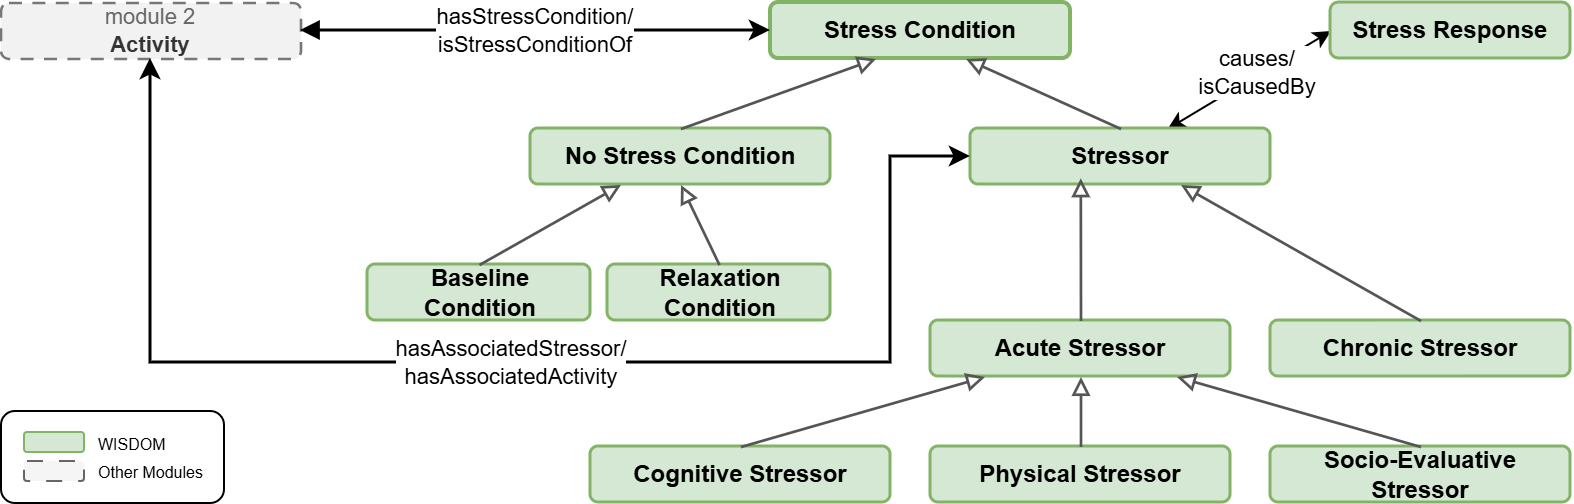
\includegraphics[width=0.9\linewidth]{images/Module1_stress_conditions.png}
    \caption{The \textit{Stress Conditions} module models the hierarchy of stress-related conditions, distinguishing stressors, non-stress conditions, and stress responses, together with their semantic relationships to activities.}
    \label{fig:module1}
\end{figure}

\textbf{Activities (Module 2).} The \textit{Activities} module represents the situational and experimental context in which stress-related conditions and observations occur (see Figure \ref{fig:module2}). Its purpose is to describe activities or phases during which a subject is exposed to a specific condition, performs a task, or is observed through sensor-based measurements. In this way, the module provides the temporal and contextual framework necessary for interpreting stress-related data. The central class of this module is \texttt{Activity}. It represents a general activity or phase that can be associated with a subject, a stress condition, and sensor-based observations. In the developed ontology, \texttt{Activity} is further specialized into different experimental or situational phases. These include \texttt{Baseline}, \texttt{PhysicalStressPhase}, \texttt{CognitiveStressPhase}, \texttt{SocioEvaluativePhase}, and \texttt{RelaxationPhase}. This structure allows the ontology to distinguish between phases that are intended to induce stress and phases that serve as non-stress or recovery-related reference states. 

The \texttt{Activity} subclasses are closely connected to the \textit{Stress Conditions} module. The object property \texttt{hasStressCondition} links an activity to the condition that characterizes it. For example, a baseline activity can be associated with a baseline condition, while a physical stress phase can be associated with a physical stressor or stress condition. In addition, the object properties \texttt{hasAssociatedStressor} and \texttt{hasAssociatedActivity} allow a direct connection between activities and stressors. This makes it possible to represent that a specific activity is not only a temporal segment, but also a context in which a particular stressor occurs.

The \textit{Activities} module is also connected to the ontology’s observation-related parts. Through the object property \texttt{hasObservation}, an activity can be linked to observations that take place during that activity. Conversely, \texttt{observedDuringActivity} allows an observation to refer back to the activity in which it was recorded. This bidirectional modeling perspective supports the contextual interpretation of sensor data, since physiological measurements can be assigned to the activity phase during which they were collected.

Temporal information is modeled using the OWL-Time ontology. Each activity is connected to a temporal \texttt{Interval} via the \texttt{time:hasTime} property, enabling the representation of its start, end, and duration. WISDOM requires every activity to be associated with at least one \texttt{Interval}. This allows activities to be linked to the corresponding time window in a data record.

In addition to these object properties, the \textit{Activities} module includes several data properties that portray descriptive characteristics of activities. The property \texttt{hasIntensity} can be used to characterize the activity’s intensity. Furthermore, \texttt{hasDescription} and \texttt{hasReference} allow activities to be documented through textual descriptions and external references. For example, a study that employs the TSST \cite{kirschbaum1993trier} as an activity to induce cognitive and socio-evaluative stress can directly refer to the original source and describe deviations from the original test through \texttt{hasDescription}.

\begin{figure}[h]
    \centering
    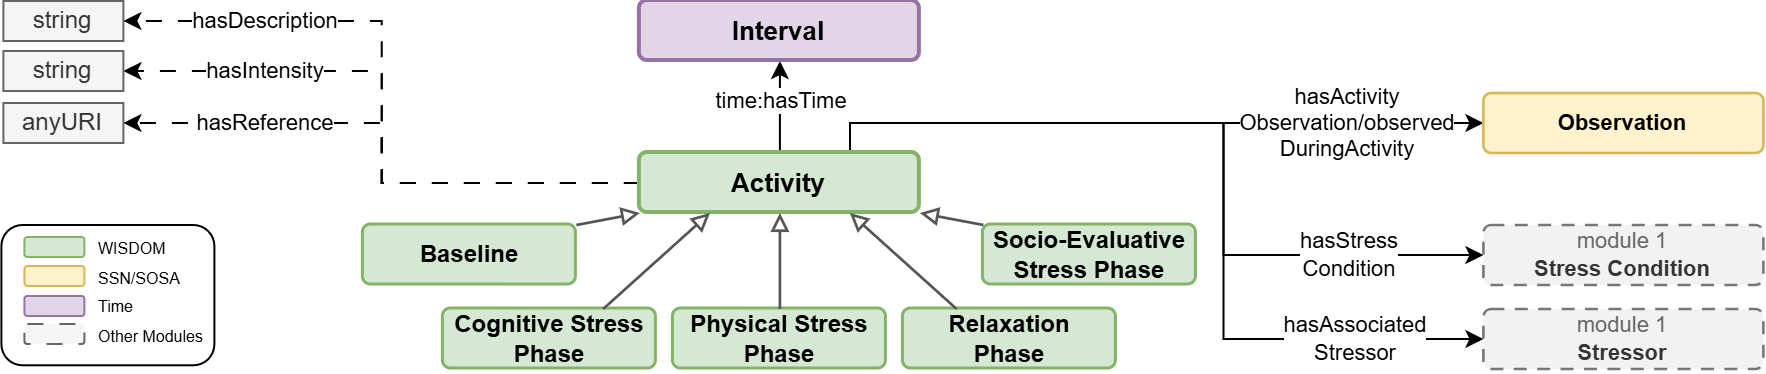
\includegraphics[width=0.9\linewidth]{images/Module2_activities.png}
    \caption{The \textit{Activities} module models experimental phases and their semantic links to stress conditions, associated stressors, and observations, providing contextual information for stress-related measurements.}
    \label{fig:module2}
\end{figure}

\textbf{Observable Properties (Module 3).} The \textit{Observable Properties} module defines the measurable characteristics that can be observed in the context of stress-related data collection (see Figure \ref{fig:module3}). Its purpose is to represent what is measured or observed, independently of the sensor or recording structure used to capture it. This distinction is important because a sensor, a signal channel, and the property being measured are conceptually different elements of the ontology. The central reference point of this module is sosa:ObservableProperty. In the developed ontology, observable properties are further differentiated into \texttt{PhysiologicalProperty}, \texttt{BehavioralProperty}, and \texttt{EnvironmentalProperty}.

The class \texttt{PhysiologicalProperty} represents measurable bodily characteristics that may be relevant for the interpretation of stress. It includes properties such as \texttt{HeartRate}, \texttt{HeartRateVariability}, \texttt{ElectrodermalActivity}, \texttt{SkinTemperature}, \texttt{BloodOxygenSaturation}, and acceleration-related properties. These properties are particularly important in wearable- and sensor-based stress research, as they provide measurable indicators of physiological activation or changes in bodily state. Therefore, they are modeled as observable indicators that require contextual interpretation.

The class \texttt{BehavioralProperty} represents observable characteristics related to behavior. In the current ontology, this includes concepts such as Gesture. Behavioral properties can complement physiological measurements by providing information about outward manifestations or movement-related aspects of a situation.

The class \texttt{EnvironmentalProperty} represents observable contextual characteristics of the environment. Examples include \texttt{Humidity} and \texttt{OutsideTemperature}. These properties are relevant because physiological signals can be influenced by environmental conditions. For example, skin temperature or electrodermal activity may be affected by the surrounding environment and should therefore not be interpreted without contextual information. By including environmental properties, the ontology supports a more differentiated interpretation of sensor-based stress data.

\begin{figure}[h]
    \centering
    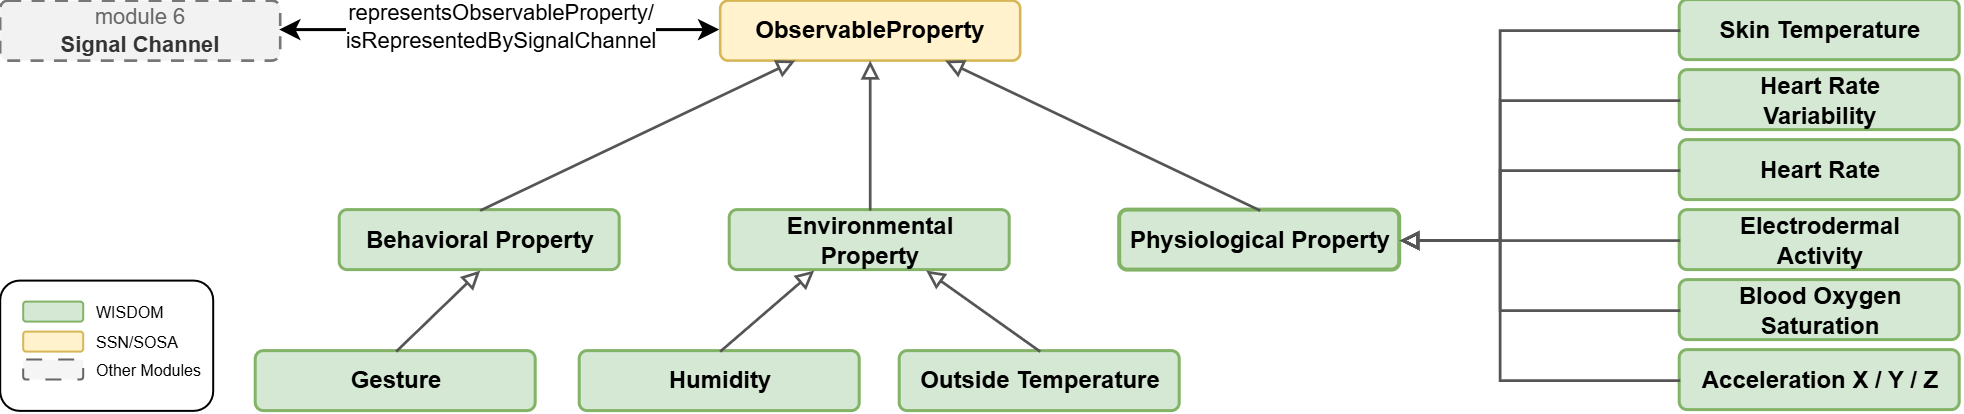
\includegraphics[width=0.9\linewidth]{images/Module3_observable_properties.png}
    \caption{The \textit{Observable Properties} module models measurable physiological, behavioral, and environmental characteristics independently of the sensors and data structures used to observe them.}
    \label{fig:module3}
\end{figure}

\textbf{Sensors (Module 4).} The \texttt{Sensors} module represents the technical components and platforms that are used to capture stress-related data (see Figure \ref{fig:module4}). Its purpose is to describe which sensors that can be hosted by instances of \texttt{WearableDevice} are involved in the observation process and how they are related to the measurable properties represented in the ontology. While the \textit{Observable Property} module defines what can be observed, the \textit{Sensors} module defines how these properties are measured.

The central reference point of this module is \texttt{sosa:Sensor}. In the developed ontology, sensor-related concepts are aligned with this class in order to follow the modeling perspective provided by SOSA/SSN. This allows sensors to be represented as entities that observe specific properties rather than as isolated technical devices. The ontology includes several sensor types that are relevant for wearable- and sensor-based stress research, including physiological sensors, motion sensors, audio sensors, and camera-based sensors. The class \texttt{PhysiologicalSensor} represents sensors that capture physiological signals relevant to stress-related processes. This includes sensor types such as \texttt{PPGSensor}, \texttt{EDASensor}, and \texttt{TemperatureSensor}. These sensors are associated with physiological properties such as heart rate, blood oxygen saturation, electrodermal activity, and skin temperature. The inclusion of these sensor types reflects the ontology’s focus on wearable-based stress representation, where physiological signals form an important basis for stress interpretation.

The class \texttt{MotionSensor} represents sensors that capture movement-related information. This includes sensors such as an accelerometer,  a gyro sensor, and a magnetometer. These sensors are relevant because movement and physical activity may influence physiological signals and, therefore, need to be considered when interpreting stress-related measurements. For example, an increase in heart rate may be caused by physical exertion rather than psychological stress. By modeling motion sensors explicitly, the ontology supports a more contextualized interpretation of physiological data.

\begin{figure}[h]
    \centering
    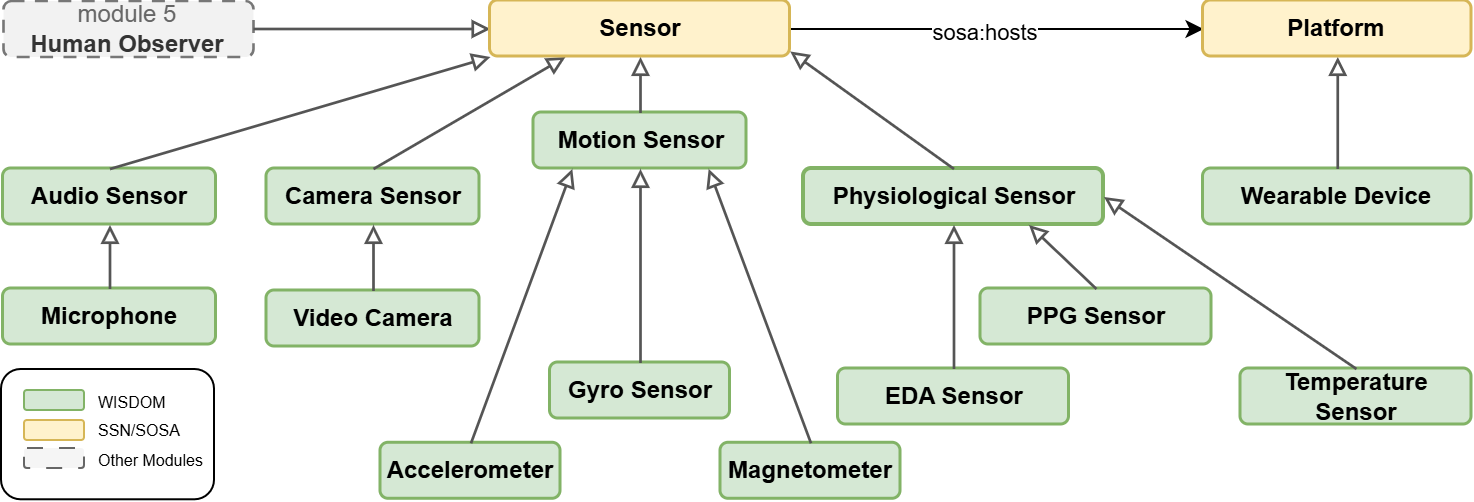
\includegraphics[width=0.85\linewidth]{images/Module4_sensors.png}
    \caption{The \textit{Sensors} module models a hierarchy of wearable sensor classes, including physiological, motion, audio, and camera sensors, and their semantic relationships to the observable properties they measure.}
    \label{fig:module4}
\end{figure}

\textbf{Person (Module 5).} The \textit{Person} module represents the human entities involved in the ontology (see Figure \ref{fig:module5}). Its purpose is to distinguish between persons in a general sense and persons who take a specific role within stress-related observations or experimental settings. This distinction is important because the ontology not only models physiological or sensor-based data, but also relates these data to the individuals from whom they are collected.
The central class of this module is \texttt{schema:Person}. It represents a human being as a general entity within the ontology. Based on this class, the ontology introduces more specific roles that are relevant in the context of stress-related data collection. The most important specialization is \texttt{Subject}, which represents a person participating in a stress-related observation, experiment, or measurement setting. A subject is therefore not modeled as a patient in a clinical sense, but as the person from whom stress-related data are collected.

The class \texttt{Subject} plays a central role in connecting the conceptual and data-oriented parts of the ontology. Since physiological measurements and observations refer to a specific person, the subject provides the human reference point for sensor-based records and observations. In this sense, the subject is the entity whose physiological, behavioral, or contextual properties are observed. This modeling perspective is aligned with the sensor-based structure of the ontology, where observations are not treated as isolated values but as measurements related to a specific feature of interest.

In addition to the subject role, the ontology also includes observer-related concepts. The class \texttt{HumanObserver}, which is further specialized into \texttt{ExperimenterObserver} allow the ontology to represent human involvement in the observation or annotation processes of an experiment, for example, when an experimenter documents an activity phase or provides additional contextual information. This is achieved through a subclass relation to \texttt{sosa:Sensor}.

\begin{figure}[h]
    \centering
    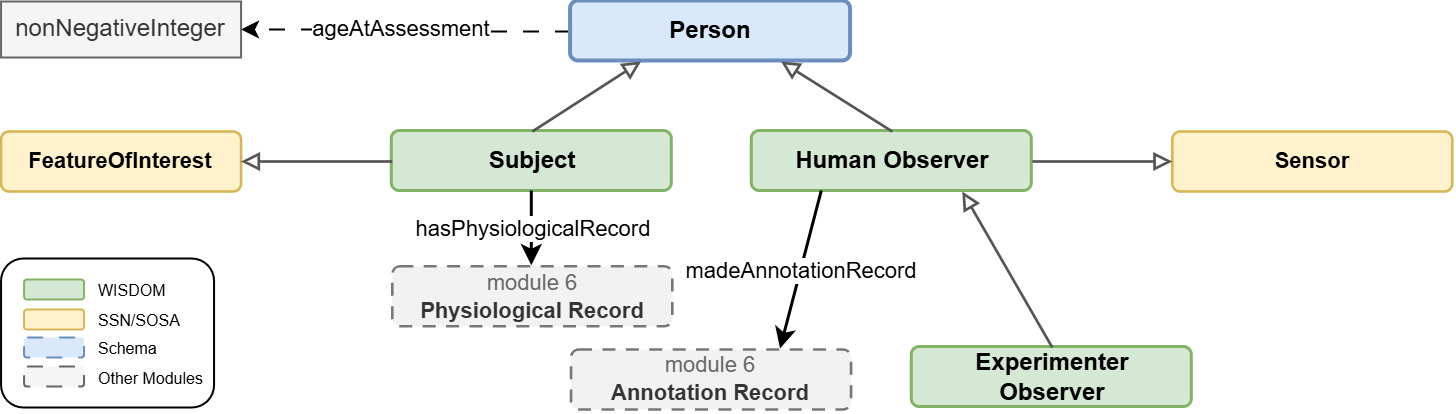
\includegraphics[width=0.9\linewidth]{images/Module5_person.png}
    \caption{The \textit{Person} module models human entities by distinguishing subjects from human observers and experimenters, defining their roles within stress-related observations and experiments.}
    \label{fig:module5}
\end{figure}

\textbf{Recordings (Module 6).} The \textit{Recordings} module represents the data-oriented part of the ontology (see Figure \ref{fig:module6}). Its purpose is to describe how sensor-based measurements are structurally organized and how individual observations are linked to persons, activities, sensors, and observable properties. This module is particularly important because wearable-based stress data are commonly not represented as isolated values, but as time-series records that contain several signal channels and observations over time.
The core classes for this module are \texttt{PhysiologicalRecord}, \texttt{AnnotationRecord} \texttt{SignalChannel} and \texttt{TimeSeriesObservation}. \texttt{PhysiologicalRecord} represents a physiological measurement record, such as a data file or recording session containing sensor-based measurements of a subject. A record can contain multiple channels, which are represented by the class \texttt{SignalChannel}. Each signal channel represents a specific stream of data within a record, such as a heart rate, electrodermal activity, temperature, or acceleration channel. An \texttt{AnnotationRecord} contains notes made by the human observer during an experiment. The class \texttt{TimeSeriesObservation} extends \texttt{sosa:Observation} to represent observations derived from wearable time-series signals. Each observation can be linked to its source record and signal channel. The class \texttt{BiomarkerAssay} represents laboratory analyses of biological samples, enabling biochemical measurements to be integrated with wearable observations.

The relation between records and channels is represented through the object property \texttt{hasSignalChannel}. This property links a \texttt{PhysiologicalRecord} to the signal channels it contains. A single measurement record may include multiple physiological or motion-related signals. By explicitly modeling channels, the ontology can represent multimodal sensor data more precisely and transparently. Each signal channel can be linked to the \textit{Observable Property} module through the object property \texttt{representsObservableProperty}. This relationship specifies which observable property is represented by a given channel. For example, a signal channel may represent heart rate or electrodermal activity. This modeling decision separates the structure of the data from the meaning of the data. A channel is therefore not treated as the physiological property itself, but as the data stream through which an observable property is represented.

\begin{figure}[h]
    \centering
    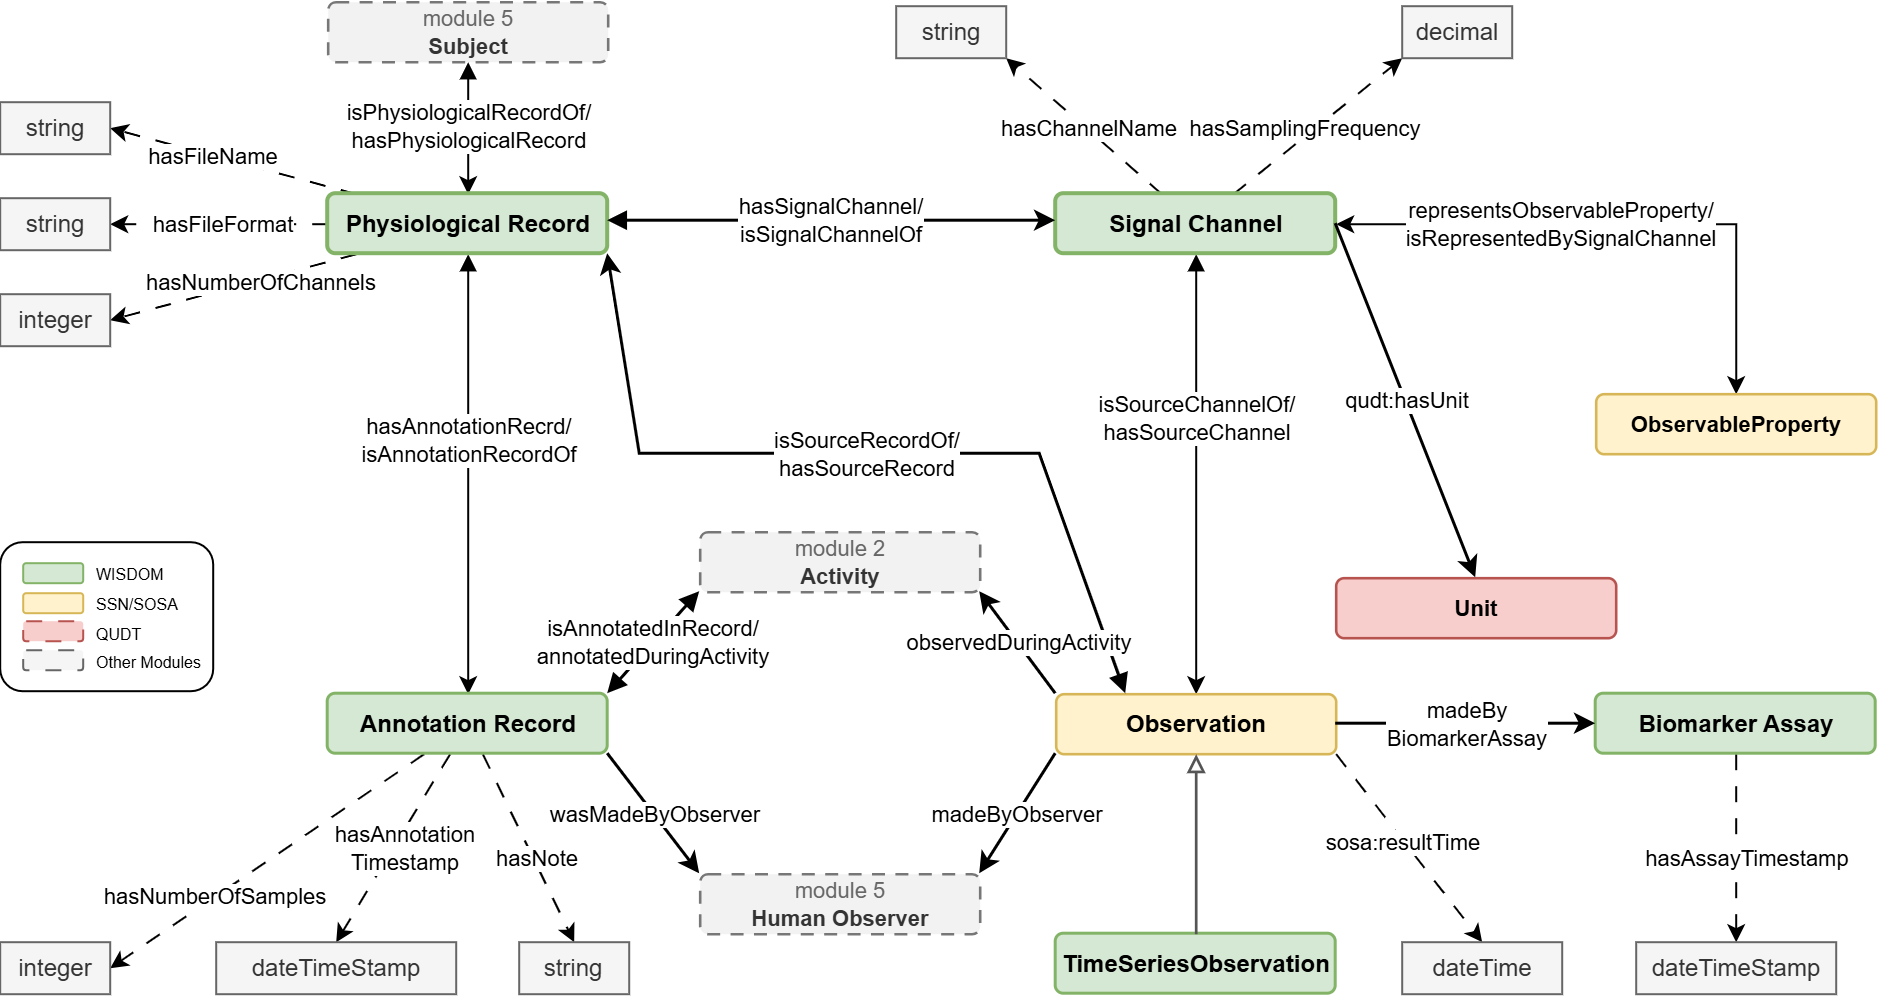
\includegraphics[width=0.9\linewidth]{images/Module6_recordings.png}
    \caption{The \textit{Recordings} module models the semantic integration of wearable measurements and human observations by linking physiological and annotation records to signal channels and time-series observations.}
    \label{fig:module6}
\end{figure}

\section{Evaluation} \label{sec:evaluation}
Besides utilizing OOPS! \cite{PovedaVillalon2014}, the WISDOM ontology was evaluated using two complementary strategies that addressed both functional adequacy and conceptual design. First, a CQ-based evaluation was conducted to verify that the ontology satisfies the requirements defined during the ontology engineering process. Second, WISDOM was compared with a set of independently AI-generated ontologies to assess how its manually engineered conceptualization related to ontology models derived from different knowledge sources. Together, these evaluation strategies provide evidence of the ontology's completeness with respect to the defined requirements and its conceptual robustness.

\subsection{Competency Questions-based and data-driven Evaluation}
CQs guided the development of WISDOM from the initial specification phase onwards and therefore served as the primary instrument for evaluating whether the final ontology fulfills its intended scope. In total, 41 CQs were iteratively developed to capture the ontology's functional requirements.

To systematically evaluate WISDOM, every CQ was manually analyzed and mapped to the ontology elements required for answering it. This verification ensured that all required concepts were explicitly represented by the final ontology and that every ontology class, object property, and data property contributed to answering at least one CQ. Consequently, the evaluation confirmed 100\% ontology coverage, indicating that all functional requirements defined during ontology development are supported.

Table \ref{tab:cqs} presents a representative subset of CQs together with the ontology elements required to answer them. The complete CQ catalog is provided as supplementary material.

% \begin{table}[h]
% \caption{CQs are opposed to the entities they are answered by. We categorized the CQs according to the subject they address: Stress Condition, Activities, Person, and Sensor. }
% \begin{tabular}{|p{2.2cm}|p{1.2cm}|p{3.5cm}|p{7.2cm}|}
% \hline
% \textbf{Module} & \textbf{CQ} &  \textbf{Question} & \textbf{Entities}\\
% \hline
% \multirow{2}{*}{Stress Condition}
%     & CQ1 & Which stress-related conditions can be distinguished? & (Stressor - subClassOf - StressCondition)\newline
%       (NoStressCondition - subClassOf - StressCondition\\
%     & CQ2 & What types of stressors can be described? & (AcuteStressor - subClassOf - Stressor)\newline
%     (ChronicStressor - subClassOf - Stressor)\\
% \hline
% \multirow{2}{*}{Activity}
%     & CQ7 & Which stressor is associated with a specific activity
%     phase? & (PhysicalStressor - hasAssociatedActivity - PhysicalStressPhase)\newline
%     (CognitiveStressor - hasAssociatedActivity - CognitiveStressPhase)\newline
%     (SocioEvaluativeStressor - hasAssociatedActivity - SocioEvaluativeStressPhase)\\
% \hline
% \multirow{2}{*}{Person}
%     & CQ9 & Which roles can a person take in the model? & (Subject - subClassOf - schema:Person)\newline
%     (HumanObserver - subClassOf - schema:Person)\newline
%     (ExperimenterObserver - subClassOf - HumanObserver)\\
% \hline
% \multirow{2}{*}{Sensor}
%     & CQ12 & Which sensor types can be used for stress-related measurements? & 
%     (PhysiologicalSensor - subClassOf - sosa:Sensor)\newline
%     (MotionSensor - subClassOf - sosa:Sensor)\newline
%     (AudioSensor - subClassOf - sosa:Sensor)\newline
%     (CameraSensor - subClassOf - sosa:Sensor)\newline
%     (HumanObserver - subClassOf - sosa:Sensor)\\
%     & CQ13 & Which physiological sensors are included? & (PPGSensor - subClassOf - PhysiologicalSensor)\newline
%     (EDASensor - subClassOf - PhysiologicalSensor)\newline
%     (TemperaturSensor - subClassOf - PhysiologicalSensor)\\
% \hline
% \end{tabular}
% \label{tab:cqs}
% \end{table}

\begin{table}[h]
\caption{CQs are opposed to the entities they are answered by. We categorized the CQs according to the subject they address: Stress Condition, Activities, Person, and Sensor.}
\label{tab:cqs}
\begingroup
\footnotesize
\setlength{\tabcolsep}{3pt}
\renewcommand{\arraystretch}{0.9}
\begin{tabular}{|p{1.5cm}|p{0.65cm}|p{3.5cm}|p{7.2cm}|}
\hline
\textbf{Module} & \textbf{CQ} & \textbf{Question} & \textbf{Entities}\\
\hline
\multirow{2}{*}{\shortstack[l]{Stress\\Condition}}
    & CQ1 & Which stress-related conditions can be distinguished?
    & (Stressor - subClassOf - StressCondition)\newline
      (NoStressCondition - subClassOf - StressCondition)\\
    & CQ2 & What types of stressors can be described?
    & (AcuteStressor - subClassOf - Stressor)\newline
      (ChronicStressor - subClassOf - Stressor)\\
\hline
Activity
    & CQ7 & Which stressor is associated with a specific activity phase?
    & (PhysicalStressor - hasAssociatedActivity - PhysicalStressPhase)\newline
      (CognitiveStressor - hasAssociatedActivity - CognitiveStressPhase)\newline
      (SocioEvaluativeStressor - hasAssociatedActivity - SocioEvaluativeStressPhase)\\
\hline
Person
    & CQ9 & Which roles can a person take in the model?
    & (Subject - subClassOf - schema:Person)\newline
      (HumanObserver - subClassOf - schema:Person)\newline
      (ExperimenterObserver - subClassOf - HumanObserver)\\
\hline
\multirow{2}{*}{Sensor}
    & CQ12 & Which sensor types can be used for stress-related measurements?
    & (PhysiologicalSensor - subClassOf - sosa:Sensor)\newline
      (MotionSensor - subClassOf - sosa:Sensor)\newline
      (AudioSensor - subClassOf - sosa:Sensor)\newline
      (CameraSensor - subClassOf - sosa:Sensor)\newline
      (HumanObserver - subClassOf - sosa:Sensor)\\
    & CQ13 & Which physiological sensors are included?
    & (PPGSensor - subClassOf - PhysiologicalSensor)\newline
      (EDASensor - subClassOf - PhysiologicalSensor)\newline
      (TemperaturSensor - subClassOf - PhysiologicalSensor)\\
\hline
\end{tabular}
\endgroup
\end{table}

To complement this conceptual evaluation, we plan to instantiate the ontology with data from real-world stress experiments involving human participants \cite{Schreiber2025} that we conducted. The resulting knowledge graph would contain representative individuals covering the central ontology modules, including subjects, stress conditions, activities, sensors, physiological records, signal channels, observable properties, observations, and annotations. The SPARQL-based validation would then extend the current confirmation of the ontology’s coverage with respect to the defined requirements by demonstrating that it can be applied in practice to query realistic stress-related data and retrieve relevant knowledge from an instantiated knowledge base.


\subsection{AI-supported Comparative Evaluation}
Recent advances in Generative AI have demonstrated considerable potential for supporting ontology engineering tasks, including concept extraction, ontology construction, refinement, and validation \cite{Shimizu2025, Li2025}. Motivated by these developments, WISDOM was additionally evaluated against a set of AI-generated ontologies to investigate how a manually engineered ontology compares with conceptual models generated automatically from different knowledge sources.

Four ontologies were independently generated using ChatGPT Pro (GPT-5.5). A common prompt structure was used across all four generations to keep the ontology-engineering task consistent while systematically varying the knowledge source. Each prompt specified the target domain as human stress in a wearable sensor-based context and instructed the model to construct an ontology by identifying relevant concepts, class hierarchies, semantic relationships, object and datatype properties, and an appropriate reuse of established vocabularies. The prompts differed only with respect to the domain information supplied to the model: semantic standards, CQs, representative stress dataset, or their combination. The complete prompts and generated ontologies are provided in the accompanying GitHub repository \footnote{\url{https://github.com/BurbachS/WISDOM}, accessed: 28.09.2026} to support reproducibility.
The first ontology was generated from established semantic standards, including SOSA/SSN and Schema.org, resulting in a standards-oriented conceptual model. The second ontology was derived exclusively from the CQs, capturing the functional requirements that guided the ontology development process. The third ontology was generated from representative stress datasets \cite{Schreiber2025} and therefore emphasizes measurement structures, experimental metadata, and recorded observations. Finally, a combined ontology was generated using all three knowledge sources simultaneously, integrating theoretical knowledge, functional requirements, and experimental evidence into a single conceptual model. Because it incorporates the complete set of available information, the combined ontology served as the primary reference for the comparative evaluation.

The generated ontologies were subsequently compared with WISDOM at the schema level using qualitative criteria covering conceptual coverage of the core semantic domain, representation of sensors, observations, and experimental data, alignment with the CQs, and indication of over- or undermodeling. The comparison was conducted manually and was intended as a conceptual comparison rather than a formal ranking of ontology quality. 

The comparison revealed a substantial degree of agreement regarding the core concepts required for wearable-based stress representation. Despite being generated from fundamentally different input sources, all AI-generated ontologies consistently identified concepts related to stress conditions, activities, physiological observations, sensors, and subjects. This convergence provides independent support for the conceptual decisions made during the development of WISDOM and suggests that these concepts constitute a stable semantic foundation for the domain.

At the same time, the comparison revealed a clear difference in modeling emphasis. The AI-generated ontologies primarily reflected the characteristics of their respective input sources: the standards-based ontology focused on established semantic modeling patterns, the CQ-based ontology emphasized functional requirements, and the dataset-based ontology concentrated on experimental structures and recorded measurements. Consequently, the combined ontology offers a broader representation of heterogeneous stress-related knowledge. In contrast, WISDOM provides a theory-driven conceptualization of stress by explicitly integrating established stress theories with sensor- and observation-oriented semantic modeling. This is particularly reflected in the explicit representation of stress conditions, stressors, contextual activity phases, and their semantic relationships.

Overall, the comparative evaluation demonstrates that manually engineered and AI-generated ontologies converge on the essential concepts required for wearable-based stress representation while pursuing different modeling strategies. Rather than identifying a superior approach, the results indicate that ontology engineering and AI-assisted ontology generation provide complementary perspectives. While the AI-generated ontologies validate many of WISDOM's modeling decisions and highlight additional modeling opportunities, WISDOM contributes a coherent, theory-driven representation of stress that remains closely aligned with established stress research. Together, these findings illustrate the potential of combining expert-driven ontology engineering with Generative AI to support the development and validation of future domains' ontologies.


\section{Conclusion and Future Work} \label{sec:conclusion}
This work introduced WISDOM, an ontology that bridges the semantic psychological representation of human stress and wearable-based sensor data commonly used to monitor physiological responses to stress. As such, in this work, we address key limitations of current ontologies that focus only on stress at a conceptual level or on sensor-based ontologies. The resulting ontology, WISDOM-Stress, provides a domain-specific semantic model that connects conceptual stress knowledge with sensor-based observations, physiological properties, activities, subjects, and contextual information. By integrating recognized standards such as QUDT, OWL-Time, SCHEMA, and SSN/SOSA, WISDOM ensures interoperability, reusability, and semantic precision.

Future work will focus on the instantiation of WISDOM with heterogeneous stress datasets and the validation of the ontology through extended SPARQL queries. Moreover, future work will also integrate WISDOM-Stress into practical stress-monitoring or data-analysis workflows. In such a scenario, the ontology serves as a semantic layer between raw wearable sensor data and data-driven analysis methods. Machine learning models can be used to classify stress-related patterns, while the ontology provides contextual information and improves the interpretability of the underlying data structures. This combination of symbolic semantic modeling and statistical analysis could be particularly relevant for explainable stress detection systems.


\section*{Declaration on Generative AI}
During the preparation of this work, the author used ChatGPT and Grammarly in order to: Grammar and spelling check, translate, paraphrase, and reword. After using these tools, the author reviewed and edited the content as needed and takes full responsibility for the publication’s content.

\section*{Resource Availability Statement} \label{sec:resources}
The WISDOM ontology\footnote{\url{https://burbachs.github.io/WISDOM/WISDOM.owl}}, the competency questions\footnote{\url{https://github.com/BurbachS/WISDOM/blob/main/CQs/CompetencyQuestions.txt}} are available on GitHub \cite{BurbachSGitHub2026} and Zenodo (DOI: \href{https://doi.org/10.5281/zenodo.21677141}{10.5281/zenodo.21677141}). All resources are licensed under \href{https://creativecommons.org/licenses/by-nc-sa/4.0/}{Creative Commons Attribution-NonCommercial-ShareAlike 4.0 International}.

\bibliography{literature.bib}


\end{document}
